% !TEX encoding = UTF-8
% !TEX TS-program = pdflatex
% !TEX root = computabilità e algoritmi.tex
% !TEX spellcheck = it-IT
\begin{figure}[htbp]
\centering
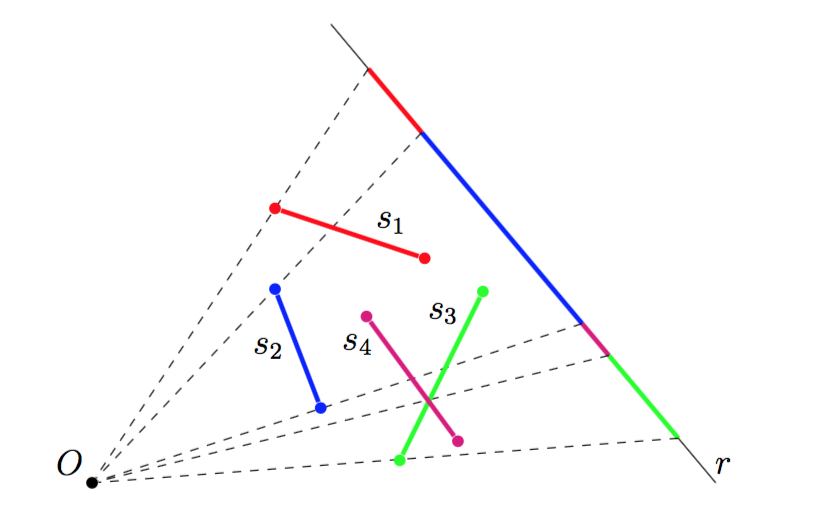
\includegraphics[width=.7\textwidth]{./notes/immagini/l36-fig1.png}
\caption{Esempio di proiezione dei segmenti}
\end{figure}

Per decidere se un segmento copre l'altro, l'idea è di confrontare a due a due i segmenti, osservando se uno si trova tutto dalla stessa parte dell'altro.

Dopodiché, se il punto di osservazione sta nel semipiano opposto al segmento, il segmento in mezzo è davanti all'altro segmento. Altrimenti se si trovano nello stesso piano, il segmento sta davanti a quello di riferimento.

Se invece i due estremi di un segmento si trovano nei due diversi semipiani, basta modificare il segmento di riferimento, tanto per
ipotesi i due segmenti non si intersecano.

\begin{breakablealgorithm}
	\caption{\textsc{Precede}: confronto tra due segmenti}
	\begin{algorithmic}[1]
\Function{Precede}{$s_1, s_2, O$}
    \State // Calcolo le posizioni degli estremi del segmento $s_2$
    \State // rispetto $s_1$
    \State $d_1 \gets \textsc{Angle-Left}(p_1, q_1, p_2)$
    \State $d_2 \gets \textsc{Angle-Left}(p_1, q_1, q_2)$
    \If{$(d_1 \geq 0 \textbf{ and } d_2 \geq 0) \textbf{ or }(d_1 \leq 0 \textbf{ and } d_2 \leq 0)$}
        \State // I due punti stanno nello stesso semipiano rispetto $s_1$
        \State $d_3 \gets \textsc{Angle-Left}(p_1,q_1, O)$
        \State \Return $(d_1 \geq 0\textbf{ and } d_2 \geq 0 \textbf{ and } d_3 \geq 0)$ \textbf{or }
        \Statex $\qquad \qquad \qquad \:(d_1 \leq 0 \textbf{ and } d_2 \leq 0 \textbf{ and } d_3 \leq 0)$
        \State // C'è un problema se $d_1 = d_2 = d_3 =0$, ovvero sono
        \State // tutti collineari, ma in questo caso si ha che la proiezione
        \State // è un punto e quindi non ci interessa.
    \Else
        \State $d_1 \gets \textsc{Angle-Left}(p_2, q_2, p_1)$
        \State $d_2 \gets \textsc{Angle-Left}(p_2, q_2, q_1)$
        \State $d_3 \gets \textsc{Angle-Left}(p_2,q_2, O)$
        \State \Return $(d_1 > 0 \textbf{ or } d_2 > 0 \textbf{ or } d_3 > 0)$ \textbf{and}
        \Statex $\qquad \qquad \qquad \:(d_1 < 0 \textbf{ or } d_2 < 0 \textbf{ or } d_3 < 0)$
    \EndIf
\EndFunction
\end{algorithmic}
\end{breakablealgorithm}

C'è un problema se $d_1 = d_2 = d_3 =0$, ovvero sono i segmenti e il punto di osservazione sono collineari, ma in questo caso si ha che la proiezione è un punto e quindi non ci interessa.

Questo test viene fatto in tempo costante e quindi tutto l'ordinamento può essere fatto in tempo $O(n \log n)$.

Una volta ordinati la proiezione dei segmenti richiede un tempo $O(n)$.

Tuttavia, se cambia il punto di osservazione è necessario effettuare un nuovo ordinamento, sarebbe bello poter avere una pre-elaborazione che permetta di risparmiare tempo. 
Questo si può fare con un albero di partizione binaria.

\subsection{Albero di partizione binaria}\label{albero-di-partizione-binaria}

Viene fissato un segmento di riferimento $s_1$ che diventa la radice dell'albero, dopodiché l'insieme dei segmenti viene partizionato rispetto $s_1$ e i segmenti che si trovano a destra di $s_1$ diventano i figli destri di $s_1$ e quelli a sinistra i figli sinistri.

Una volta costruito l'albero, basta guardare dove si trova il punto di osservazione rispetto al segmento $s_1$, se ad esempio si trova a
destra, è necessario prima proiettare la partizione sinistra, poi $s_1$ ed infine la partizione destra.

La funzione proietta risulterà essere

\begin{breakablealgorithm}
	\caption{\textsc{Proietta}: proiezione utilizzando l'albero di partizionamento}
	\begin{algorithmic}[1]
\Function{Proietta}{$x,O$}
    \If{$x \neq \textsc{Nil}$}
        \State // $x$ nodo radice con etichetta il segmento $x.s = \overline{pq}$
        \State $d \gets \textsc{Turn-Left}(p,q,O)$
        \If{$d \geq 0$}
            \State // $O$ appartiene al semipiano positivo
            \State \textsc{Proietta}(x.left,O)
            \State \textsc{Disegna}(x.s)
            \State \textsc{Proietta}(x.right,O)
        \Else
            \State \textsc{Proietta}(x.right,O)
            \State \textsc{Disegna}(x.s)
            \State \textsc{Proietta}(x.left,O)
        \EndIf 
    \EndIf
\EndFunction
\end{algorithmic}
\end{breakablealgorithm}

Così facendo la proiezione richiede $O(n)$ moltiplicato per una costante molto piccola.

C'è però un problema se c'è un segmento a cavallo dei due piani che deve essere risolto andando a spezzare il segmento in due segmenti, in modo che ognuno dei due si trovi in un semipiano diverso.

\begin{figure}[htbp]
\centering
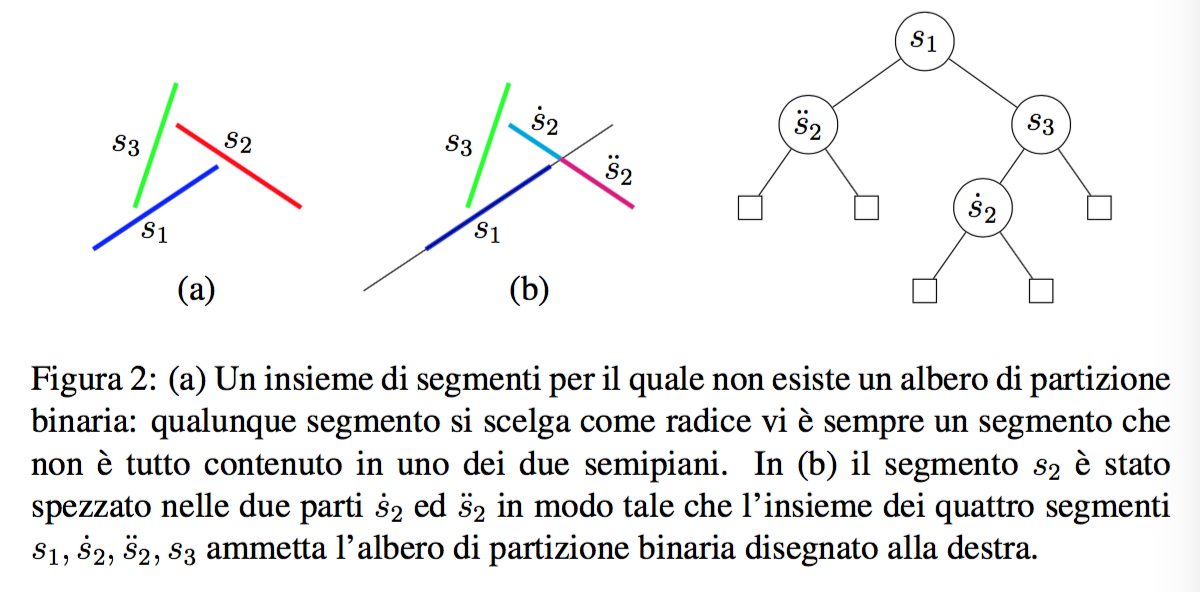
\includegraphics[width=.7\textwidth]{./notes/immagini/l36-fig2.png}
\end{figure}

L'albero di partizione binaria può essere quindi costruito con

\begin{breakablealgorithm}
	\caption{\textsc{Partizione-Binaria}: costruzione dell'albero di partizione binaria}
	\begin{algorithmic}[1]
\Function{Partizione-Binaria}{S, n}
    \If{$n = 0$}
        \State \Return \textsc{Nil}
    \EndIf
    \State // Divide il piano rispetto il segmento $s_1$
    \State $npos, nneg \gets 0$
    \For{$i = 2 \textbf{ to } n$}
        \If{$s_i$ è tutto nel semipiano positivo}
            \State $npos \gets npos+1$
            \State $Spos[npos] \gets s_i$
        \ElsIf{$s_i$ è tutto nel semipiano negativo}
            \State $nneg \gets nneg+1$
            \State $Sneg[nneg] \gets s_i$
        \Else
            \State Dividi $s_i$ in due parti $s_i'$ e $s_i''$ usando la retta $s_1$.
            \State $npos \gets npos+1$
            \State $Spos[npos] \gets s_i'$
            \State $npos \gets npos+1$
            \State $Spos[npos] \gets s_i''$
        \EndIf
    \EndFor
    \State $x.s \gets s_1$
    \State $x.left \gets \textsc{Partizione-Binaria}(Sneg, nneg)$
    \State $x.right \gets \textsc{Partizione-Binaria}(Spos, npos)$
    \State \Return $x$
\EndFunction
\end{algorithmic}
\end{breakablealgorithm}

Per dividere un segmento in due parti mantenendo le coordinate intere è possibile prendere i due punti più vicini all'intersezione dei due
segmenti.

\subsection{Randomizzazione della partizione}\label{randomizzazione-della-partizione}

C'è però un problema: spezzando i segmenti, \emph{n} aumenta e di conseguenza aumenta il tempo anche per effettuare la proiezione.

Nel caso pessimo si ha che considerando l'insieme di segmenti $s_i = (p_i, q_i)$ tali che $p_i = (i,0)$ e $q_i = (i+1, 2^{i+1}-1)$, ovvero una situazione simile a

\begin{figure}[htbp]
\centering
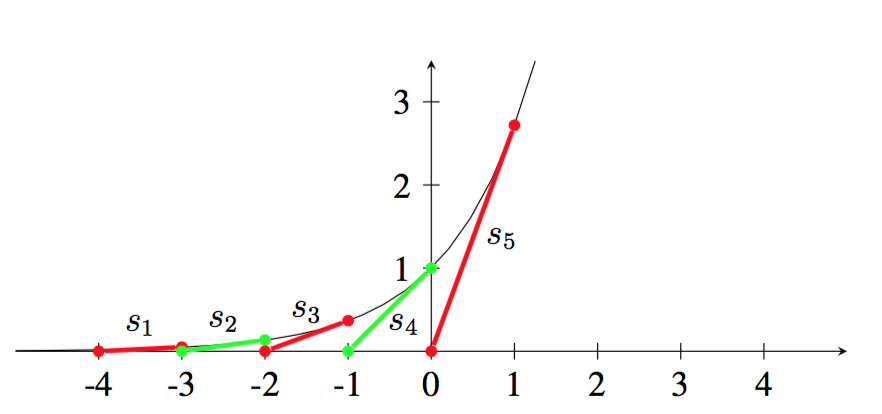
\includegraphics[width=.7\textwidth]{./notes/immagini/l36-fig3.png}
\caption{La curva non è proprio quella ma il concetto è lo stesso}
\end{figure}

Con questo insieme, se viene scelto come primo segmento $s_1$ è necessario partizionare più volte tutti gli altri segmenti, mentre se
prendo $s_n$ non serve effettuare nessuna divisione.

Siccome non è sempre detto che partire dall'ultimo sia sempre la cosa migliore, l'idea è quindi quella di randomizzare l'ordine dei segmenti
prima di effettuare la partizione.

\begin{breakablealgorithm}
	\caption{\textsc{Random-Partizione-Binaria}: partizione binaria casuale}
	\begin{algorithmic}[1]
	\Function{Random-Partizione-Binaria}{$S,n$}
	    \State // Ri-ordina casualmente $S$
	    \State \Return \textsc{Partizione-Binaria}$(S,n)$
	\EndFunction
\end{algorithmic}
\end{breakablealgorithm}

Così facendo si ha che il valore atteso del numero di nodi (segmenti) è $O(n \log n)$.

\subsubsection{Dimostrazione}\label{dimostrazione}

\begin{figure}[htbp]
\centering
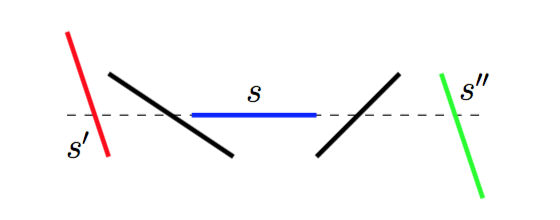
\includegraphics[width=.7\textwidth]{./notes/immagini/l36-fig4.png}
\end{figure}

Se il segmento \emph{s} taglia un segmento \emph{s'}, la distanza $d(s,s') = k$ è definita come il numero di segmenti che la retta passante per \emph{s} taglia prima di tagliare \emph{s'}. $d(s,s')=\infty$ se non lo taglia.

Supponendo quindi che la retta passante per $s$ tagli il segmento $s'$ a distanza $k$, si ha che durante l'esecuzione dell'algoritmo, il segmento $s'$ viene tagliato solo se il segmento $s$ viene scelto prima di tutti gli altri segmenti $s_1, s_2, s_{k-1}, s'$ e la probabilità che questo succeda è minore o uguale $1/(k+1)$. 
Il minore o uguale deriva dal fatto che il segmento \emph{s'} può essere già stato tagliato da un segmento, inoltre, per definizione, se \emph{s} non taglia \emph{s'}, $d(s,s') = \infty$ e quindi la probabilità di taglio risulta essere 0.

Sia $X_{s,s'}$ la variabile casuale che vale 0 se \emph{s} non suddivide \emph{s'} e vale 1 altrimenti.

Per costruzione il valore atteso di $X$ è uguale alla probabilità di taglio:

$$
E[X_{s,s'}] \leq \frac{1}{d(s,s') +1}
$$

Il numero \emph{m} di nodi dell'albero di partizione è dato dal numero di segmenti \emph{n} di partenza più il numero di suddivisioni
effettuate

$$
m = n + \sum\limits_{s} \sum\limits_{s' \neq s}X_{s,s'}
$$

Il valore atteso di \emph{m} è risulta quindi essere

$$
\textbf{E}[m] = E\Bigg[n + \sum\limits_{s} \sum\limits_{s' \neq s}X_{s,s'} \Bigg] = n + \sum\limits_{s} \sum\limits_{s' \neq s} E[X_{s,s'}] \leq n + \sum\limits_{s} \sum\limits_{s' \neq s}  \frac{1}{d(s,s')+1}
$$

Ma si può dire di più: fissato un segmento \emph{s} e una certa distanza \emph{k} , ci sono al più due segmenti \emph{s'} e \emph{s''} che si
trovano a distanza \emph{k} da \emph{s}. 
Si ha quindi che

$$
\sum\limits_{s' \neq s} \frac{1}{d(s,s')+1} \leq \sum\limits_{k=1}^{n-1} \frac{2}{k+1} \leq 2H_n
$$

dove $H_n$ è l'\emph{n}-esimo numero armonico ($H_n = 1 + 1/2 + 1/3 + \ldots + 1/n$).

Mettendo tutto assieme si ha che

$$
\textbf{E}[m] \leq n + 2nH_n
$$

e siccome la serie armonica converge a $O(\log n)$, si ha che il valore atteso del numero di nodi va con $O(n \log n)$.

\section{Instradamento dei messaggi in un calcolatore parallelo}\label{instradamento-dei-messaggi-in-un-calcolatore-parallelo}

Abbiamo una rete di processori che funzionano in modo parallelo che può essere rappresentata da un grafo fortemente connesso.

Assumiamo che i canali di comunicazione siano sincroni, ovvero che ad ogni istante di tempo un processore può inviare un pacchetto per ogni suo canale di uscita e riceverne uno da ogni canale in ingresso.

Ad un certo istante c'è il processore \emph{i} che invia un pacchetto $p_i$ ad un processore di destinazione $d_i$. 
Una prima idea è quella di far girare il pacchetto sul cammino minimo, ma questo può causare un problema, perché un processore potrebbe ricevere più pacchetti da instradare contemporaneamente sullo stesso canale. 
\`{E} quindi necessario che i canali siano dotati di un \textbf{buffer} in grado da tenere in memoria al coda dei pacchetti.

Si perdere quindi la garanzia del tempo di trasmissione costante, perché dipende dalla coda nel canale di comunicazione.

Consideriamo quindi il caso in cui tutti i processori \emph{i} inviino un pacchetto $p_i$ ad un altro processore $d_i$, assumendo che i vari $d_i$ siano tutti distinti, ovvero le destinazioni $d_i$ sono una permutazione delle sorgenti \emph{i} (\textbf{problema di instradamento di una permutazione}).

Riguardo a questo problema c'è il \textbf{teorema di Valiant}: sia \emph{R} una rete di \emph{n} processori tale che ogni processore abbia al più \emph{k} canali di output. 
Per ogni algoritmo di routing deterministico, esiste una permutazione $d_1 \ldots d_n$ tale che il numero di passi per far arrivare a destinazione tutti gli \emph{n} pacchetti è $\Omega(\sqrt{n/k})$ (limitato inferiormente).

Ad esempio se ci sono $2^{32}$ processori, con $k = 32$ si ha che il numero di passi è almeno $\sqrt{2^{32} /32} = 11585$ e considerando che in un iper-cubo di grado 32 (la rete descritta), il cammino più lungo è di 32 archi.
